%%%%%%%%%%%%%%%%%%%%%%%%%%%%%%%%%%%%%%%%%
% Minimalist Book Title Page 
% LaTeX Template
% Version 1.0 (27/12/12)
%
% This template has been downloaded from:
% http://www.LaTeXTemplates.com
%
% Original author:
% Peter Wilson (herries.press@earthlink.net)
%
% License:
% CC BY-NC-SA 3.0 (http://creativecommons.org/licenses/by-nc-sa/3.0/)
% 
% Instructions for using this template:
% This title page compiles as is. If you wish to include this title page in 
% another document, you will need to copy everything before 
% \begin{document} into the preamble of your document. The title page is
% then included using \titleTH within your document.
%
%%%%%%%%%%%%%%%%%%%%%%%%%%%%%%%%%%%%%%%%%

%----------------------------------------------------------------------------------------
%	PACKAGES AND OTHER DOCUMENT CONFIGURATIONS
%----------------------------------------------------------------------------------------

% packages
\documentclass[12pt,a4paper,twoside]{article}

\usepackage[svgnames]{xcolor} % Required to specify font color

\newcommand*{\plogo}{\fbox{$\mathcal{PL}$}} % Generic publisher logo


\usepackage[utf8]{inputenc}
%\usepackage[latin1]{inputenc} 
\usepackage[T1]{fontenc}
\usepackage{lmodern} % load a font with all the characters
\usepackage{gensymb}
\usepackage{mathtools,xparse}

\usepackage{amsthm}

\usepackage{amsmath}

\usepackage{amssymb}
\usepackage{pdfpages}
\usepackage{mathrsfs}

\usepackage{graphicx}

\usepackage{hyperref}

% inclure the numéro du chapitre dans les équations
\numberwithin{equation}{subsection}

\DeclarePairedDelimiter{\abs}{\lvert}{\rvert}
\DeclarePairedDelimiter{\norm}{\lVert}{\rVert}


%----------------------------------------------------------------------------------------
%	TITLE PAGE
%----------------------------------------------------------------------------------------

\newcommand*{\titleTH}{\begingroup % Create the command for including the title page in the document
\raggedleft % Right-align all text
\vspace*{\baselineskip} % Whitespace at the top of the page

{\Large Mohamed Thebti}\\[0.167\textheight] % Author name

{\LARGE\bfseries Résumé de cours}\\[\baselineskip] % First part of the title, if it is unimportant consider making the font size smaller to accentuate the main title

{\textcolor{Red}{\Huge de l'ingénierie}}\\[\baselineskip] % Main title which draws the focus of the reader

{\Large \textit{A predictable tagline}}\par % Tagline or further description

\vfill % Whitespace between the title block and the publisher

{\large The Publisher \plogo}\par % Publisher and logo

\vspace*{3\baselineskip} % Whitespace at the bottom of the page
\endgroup}

%----------------------------------------------------------------------------------------
%	BLANK DOCUMENT
%----------------------------------------------------------------------------------------

\begin{document} 
% \pagestyle{empty} % Removes page numbers

\titleTH % This command includes the title page


% indentation des paragraphes
\setlength{\parindent}{0cm}

\newpage
\tableofcontents

\newpage
\section{Introduction}

cet oeuvrage est un résumé. 

faire le lien entre différentes sciences.

Des résultats développés dans une partie sont utilisés dans d'autres parties.

\newpage
\section{Algèbre}

\subsection{Logarithme}
\subsubsection{Relations}
Fonction et fonction inverse (réciproque)
\begin{eqnarray}
e^n=x\\
ln(x)=n\\
ln(x^a)=a\cdot n
\end{eqnarray}

\subsubsection{Changement de base}
\begin{eqnarray}
log_{n}(x)=\frac{ln(x)}{ln(n)}=a\\
n^a=x
\end{eqnarray}

\subsection{Produits remarquables}
Théorème de Binôme : 
\begin{equation}
(a+b)^n=\sum_{k=0}^{n}a^{n-k}b^k
\end{equation}
\subsection{Equation de degré 2}
\begin{equation}
a x^2+ bx +c =0
\end{equation}

Discriminant

\begin{equation}
\Delta = b^2-4\cdot a \cdot c
\end{equation}

3 possibilités : 

\begin{enumerate}
	\item $\Delta > 0 $ :  Il y a deux solutions réelles.\\ $x_{1,2}=\frac{-b \pm \sqrt{\Delta}}{2 a}$
	\item $\Delta = 0 $ : Une solution réelle.
	$x=\frac{-b}{2 a}$
	\item $\Delta < 0 $ : Il y deux solutions complexes.\\
	$x_{1,2}=\frac{-b\pm i \sqrt{\abs{\Delta}}}{2 a}$
\end{enumerate}
\subsection{Equation degré 3 : Méthode de Cardan}

Inverse d'une matrice :

Produit de convolution

\subsection{Suites \& Séries}

suite de finonesci//
suite arithmétique

\begin{equation}
\sum_{k=1}^{n}k=\frac{n(1+n)}{2}
\end{equation}
\begin{equation}
\lim \frac{1-r^n}{1-r}
\end{equation}

\subsection{Nombres complexes}

\subsubsection{Utilité}
résoudre des équations qui donne des réusltats impossible dans le domaine réel. exemple $\sqrt{-1}$.\\
\subsubsection{Définition}
Partie réelle, partie imaginaire,\\

Multiplication par le conjugué\\

\subsubsection{Résolution d'équations imaginaires}

\subsection{Série et transformée de Fourier}
Continue :
\begin{equation}
F(\nu)=\int_{-\infty}^{\infty} f(t) e^{-2 i \pi \nu t} dt
\end{equation}

Discrète : 

\subsection{Transformée de Laplace}

\newpage
\section{Equations différentielles}
degré 1,2, solution homogène, solution particulière,
coefficients constants/variables. 
equ diff partielle : résolution avec fourier/Laplace

\newpage
\section{Algèbre linéaire}
\begin{equation}
A^{-1}=()
\end{equation}

décomposition LU, \\
Equation caractéristique, vecteur propre, valeur propre

\newpage
\section{Analyse numérique}

Dérivée numérique, intégrale numérique, equation différentielle partielle numérique (espace, temps), résolution , précision, \\

progressive, rétrograde

\newpage
\section{Cinématique multi-corps}
Euler, Newton\\
\\
\subsection{Résolutions des systèmes du type quadrilatère articulé}
système fait de quatre barres. 
four-bars-systems : one bar is called the "bâti". the 3 others have degrees of freedom. 

\subsubsection{Boucle vectorielle fermée}

\subsubsection{Méthode de Newton-Raphson}
Methode newton

Converge si le point de départ est assez proche du zéro

Or dans notre situation, la fonction de contrainte est très faible et le vecteur q0 est justement proche du zero de la fonction. Les valeurs de ce vecteur sont choisis avec une bonne estimation assez proches des vraies valeurs
Donc pas de problème de convergence
Le situation de depart est une position réelle, et on connait les valeurs initiales des angles et leurs intervalles


\subsubsection{equilibrage des arbres}

\section{Dynamique multi-corps}
Force centifuge
\begin{equation}
\vec{F}_{ce}=\vec{\omega}\otimes(\vec{\omega}\otimes \vec{v})
\end{equation}

Force de Coriolis : 
\begin{equation}
\vec{F}_{co}=2 \cdot \vec{\omega}\otimes \vec{v}
\end{equation}
\newpage

\newpage
\section{Cryptologie}
cours Collège\\
Codage numérique :\\
\url{https://fr.wikipedia.org/wiki/Fonction_OU_exclusif}\\

\newpage
\section{Systèmes de coordonnées}
coordonnées cartésiennes, polaires, cylindriques, sphériques, ....\\
\subsection{Coordonnées cylindriques}
\begin{eqnarray}
r=\rho \cdot \vec{e}_{\rho}+z \cdot \vec{e}_z\\
v=\dot{\rho} \cdot \vec{e}_{\rho} + \rho \cdot \dot{\Phi}\cdot \vec{e}_{\Phi}+\dot{z}\cdot \vec{e}_z\\
a=(\ddot{\rho}-\rho \cdot \Phi^2)\vec{e}_{\rho}+(\rho \cdot \ddot{\Phi}+2 \cdot \dot{\rho}\cdot \dot{\Phi})\vec{e}_{\Phi}+\dot{z}\cdot \vec{e}_z
\end{eqnarray}

\subsection{Coordonnées sphériques}

\begin{eqnarray}
r=r \cdot \vec{e}_r\\
v=r \cdot \vec{e}_{r} + r \cdot \dot{\theta}\cdot \vec{e}_{\theta}+r \cdot \Phi\cdot sin(\theta) \cdot \vec{e}_{\Phi}\\
a=(\ddot{r}-r \cdot \dot{\theta}^2-r\cdot \dot{\Phi}^2 \cdot sin^2(\theta))\vec{e}_{r}+\\
(r \cdot \ddot{\theta}+2 \cdot \dot{r}\cdot \dot{\theta}-r\cdot \dot{\theta}^2 \cdot sin(\theta)cos(\theta))\vec{e}_{\theta}+\\
(r \cdot \ddot{\Phi} \cdot sin(\theta)+2 \cdot \dot{r} \cdot \dot{\Phi} \cdot sin(\theta)+2 \cdot r \cdot \dot{\Phi} \cdot \dot{\theta} \cdot cos(\theta))\cdot \vec{e}_{\Phi}
\end{eqnarray}

\subsection{Autres systèmes de coordonnées}
système de Frenet-Seré
...
\newpage
\section{Géométrie}



\subsection{Trigonométrie}
relations
\begin{eqnarray}
cos^2(x)+sin^2(x)=1\\
\frac{cos(x)}{sin(x)}
\end{eqnarray}
\begin{equation}
tan(x)=\frac{cos(x)}{sin(x)}
\end{equation}

\begin{equation}
cotan(x)=\frac{1}{tan(x)}
\end{equation}

Thm du sinus + (schéma du triangle)
\begin{equation}
\frac{a}{sin(\alpha)}=\frac{b}{sin(\beta)}=\frac{c}{sin(\gamma)}
\end{equation}
Thm cosinus
\begin{equation}
c^2=a^2+b^2-2 \cdot a \cdot b \cdot cos(\gamma)
\end{equation}

\subsection{Triangle}
Propriétés : \\
\begin{equation}
\alpha+\beta+\gamma=\pi
\end{equation}


\subsubsection{Triangle quelconque}


Théorème d'Al-Kashi



Triangle avec cotés a,b,c et angles $\alpha$ $\beta$ $\gamma$. $\alpha$ opposé à a, $\beta$ à b, $\gamma$ à c. 
\begin{equation}
\frac{b}{a}=\frac{\beta}{\alpha}....
\end{equation}
Théorème du sinus
\begin{equation}
\frac{a}{sin(\alpha)}=\frac{b}{sin(\beta)}=\frac{c}{sin(\gamma)}=2\cdot r
\end{equation}
$r$ : rayon du cercle circonscrit. 
Théorème du cosinus
\begin{equation}
a^2=b^2+c^2 - 2 b c cos(\alpha)
\end{equation}

Aire du triangle
\begin{equation}
S=\frac{1}{2}\cdot a b sin(\gamma)=2r^2sin(\alpha)sin(\beta)sin(\gamma)
\end{equation}
\subsubsection{Triangle rectangle}

Pour vérifier qu'un triangle ABC est rectangle en un point C, on vérfie que le produit scalaire de AC et BC soit nulle


\begin{equation}
\mid \mid \vec{a}\mid \mid =
\end{equation}
\subsection{Vecteurs}
Une grandeur qui a une direction, un sens et une intensité
\begin{equation}
\vec{AB}=\vec{OB}-\vec{OA}=
\begin{bmatrix}
x_B-x_A \\
y_B-y_A\\
z_B-z_A
\end{bmatrix}
\end{equation}
Norme vecteur
\begin{equation}
\norm{\vec{B}}=\sqrt{x_B^2+y_B^2+z_B^2}
\end{equation}
Vecteur dimension n :
\begin{equation}
\norm{\vec{B}}=\sqrt{x_B^2+y_B^2+z_B^2}
\end{equation}
\begin{equation}
\norm{\vec{u}}=\sqrt{\sum_{1}^{n}u_i^2}
\end{equation}
normalisation d'un vecteur : on modifier un vecteur de façon à ce que sa norme valle 1 :

\begin{equation}
\vec{B}_{normalisé}=\frac{\vec{B}}{\norm{\vec{B}}}= \frac{1}{\sqrt{x_B^2+y_B^2+z_B^2}} \begin{bmatrix}
x_B\\
y_B\\
z_B
\end{bmatrix}
\end{equation}

Multiplication par un scalaire : 
\begin{equation}
k\cdot \vec{B}= \begin{bmatrix}
k\cdot x_B\\
k\cdot y_B\\
k\cdot z_B
\end{bmatrix}
\end{equation}
Distributivité 
\begin{equation}
k\cdot (\vec{A}+\vec{B})=k\cdot \vec{A}+k\cdot\vec{B}=
\end{equation}

Le vecteur $\vec{v}$ est colinéaire à $\vec{u}$ s'il existe un scalaire $k$ tel que :  
\begin{equation}
\vec{v}=k\cdot \vec{u}
\end{equation}

Combinaison linéaire
\begin{equation}
\vec{u}=\sum_{1}^{n} n_i \cdot \vec{x_i}
\end{equation}
3 vecteurs coplanaires : un des vecteurs est la combinaison linéaire des deux autres


\subsection{Produit scalaire}
Projection d'un vecteur sur un autre.

\begin{eqnarray}
\vec{A} \cdot \vec{B}=\norm{\vec{A}} \cdot \norm{\vec{B}} \cdot cos(\theta)\\
\vec{A} \cdot \vec{B}= 
\begin{bmatrix}
x_A \\
y_A\\
z_A
\end{bmatrix}
\begin{bmatrix}
x_B \\
y_B\\
z_B
\end{bmatrix}
=x_A x_B + y_A y_B + z_A z_B
\end{eqnarray}

Si deux vercteurs sont perpendiculaires, $theta$ vaut 90$\degree$ :
\begin{equation}
\vec{A} \cdot \vec{B}=0
\end{equation}

\subsection{Volume}
\subsection{Base}
des vecteurs forment une base s'ils sont linéairement indépendants. (non colinéaire)

\subsection{Norme}
Norme euclidienne, et les autres types de normes
\subsection{Produit vectoriel}

\subsubsection{Définition}
Le produit vectoriel de deux vecteurs $\vec{A}$ et $\vec{B}$ résulte en un vecteur qui leur est perpendiculaire. La norme de ce vecteur est égale à l'aire du parallélogramme formé par les vecteurs $\vec{A}$ et $\vec{B}$. (schéma)
\subsubsection{Relation}
\begin{eqnarray}
\vec{A} \otimes \vec{B}=\norm{A} \norm{B} sin(\theta)\\
\vec{A} \otimes \vec{B}=
\begin{bmatrix}
x_A \\
y_A\\
z_A
\end{bmatrix}
\otimes
\begin{bmatrix}
x_B \\
y_B\\
z_B
\end{bmatrix}= 
\begin{bmatrix}
y_A z_B - z_A y_B \\
-x_A z_B + z_A x_B\\
x_A y_B - y_A x_B
\end{bmatrix}
\end{eqnarray}

Pour connaître la direction du vecteur résultant, on utilise la règle des trois doigts. 

Si les deux vecteurs sont parallèles, l'angle , 
\begin{equation}
\vec{A} \otimes \vec{B}=0
\end{equation}


\subsubsection{Propriétés}
pas commutatif,
\begin{eqnarray}
\vec{A} \otimes \vec{B}=-(\vec{B} \otimes \vec{A})\\
\end{eqnarray}
distributif par rapport à l'addition, \\

pas associatif

\subsection{Equations dans l'espace}
\subsubsection{Dans le plan}
Equation paramétrique d'une droite\\
\begin{equation}
ax+by+c=0\\
\end{equation}
Equation paramétrique d'une droite\\
\begin{equation}
y=a\cdot x+b\\
\end{equation}


Forme usuelle : 
\begin{equation}
ax+by+c=0\\
\end{equation}


Equation algébrique d'une droite :
\begin{equation}
D=\{(x,y) \in \mathbb{R} ^2 |ax+by+c=0\}
\end{equation}

\subsubsection{Dans l'espace}
\paragraph{Droite}
Equation algébrique d'une droite :

\begin{equation}
D={(x,y,z) \in \mathbb{R} ^3 |ax+by+cz+d=0}
\end{equation}

Equation vectorielle d'une droite :

\begin{eqnarray}
\left\{
\begin{array}{l c c r}   
x &=& a t+ x_P &\\
y &=& b t+ x_P & \\
z &=& c t + z_P & 
\end{array}\right.
t \in \mathbb{R}
\end{eqnarray}
Avec 
$P=
\begin{bmatrix}
x_p \\
y_P\\
z_P
\end{bmatrix}
$ 
un point de la droite et $\vec{u}=\begin{bmatrix}
a\\ b\\ c
\end{bmatrix}$ vecteur directeur de la droite.\\

Une autre forme de l'équation vectorielle :

\begin{equation}
(D_1):
\begin{bmatrix}
x \\
y\\
z
\end{bmatrix}
=
\begin{bmatrix}
x_p\\
y_p\\
z_p\\
\end{bmatrix}
+
\lambda
\begin{bmatrix}
a\\
b \\
c
\end{bmatrix}
; \lambda \in \mathbb{R}
\end{equation}
\paragraph{Plan}
Equation paramétrique d'un plan :
\begin{equation}
ax+bx+cz+d=0
\end{equation}
Avec $\vec{u}=\begin{bmatrix}
a\\ b\\ c
\end{bmatrix}$ verteur normale au plan.\\
Equation vectorielle :
\begin{equation}
(\Pi):
\begin{bmatrix}
x \\
y\\
z
\end{bmatrix}
=
\begin{bmatrix}
x_p\\
y_p\\
z_p\\
\end{bmatrix}
+\lambda
\begin{bmatrix}
m_1\\
m_2 \\
m_3
\end{bmatrix}
+ \gamma
\begin{bmatrix}
n_1\\
n_2 \\
n_3
\end{bmatrix}; (\lambda,\gamma) \in \mathbb{R}
\end{equation}
$\vec{m}$ et $\vec{n}$ appartiennent au plan $\Pi$.
\paragraph{Cercle}

\begin{equation}
r^2=x^2+y^2
\end{equation}
Paramétrisation :
\begin{equation}
C =
\begin{bmatrix}
r \cdot cos(\theta) \\
r \cdot sin(\theta)\\
z
\end{bmatrix}
\end{equation}
Equation cercle, sphère, couronne, solénoide, courbes, splines, ....\\

résumer le tout dans un tableau. 

\subsection{Allignements}
pour vérifier si des points sont alignés, il y a deux méthodes :\\
Méthode 1 : 
\begin{enumerate}
	\item Calculer les vecteurs directeurs entre chaques deux points
	\item Normaliser ces vecteurs
	\item Comparer
	\item Les vecteurs normalisés doivent être égaux
\end{enumerate}

Méthode 2 : 
\begin{enumerate}
	\item Choisir deux points
	\item Créer une droite avec une équation vectorielle
	\item Vérifier que les autres points appartiennent à la droite
\end{enumerate}

\subsection{Intersections}
Intersection entre deux éléments : égaliser les expressions.
\medbreak
Exemple : soit deux droites $D_1$ et $D_2$ :
\begin{equation}
(D_1):
\begin{bmatrix}
x \\
y\\
z
\end{bmatrix}
=
\begin{bmatrix}
x_p\\
y_p\\
z_p\\
\end{bmatrix}
+
\lambda
\begin{bmatrix}
a\\
b \\
c
\end{bmatrix}
; \lambda \in \mathbb{R}
\end{equation}
\begin{equation}
(D_2):
\begin{bmatrix}
x \\
y\\
z
\end{bmatrix}
=
\begin{bmatrix}
u_p\\
v_p\\
w_p\\
\end{bmatrix}
+
\gamma
\begin{bmatrix}
d\\
e \\
f
\end{bmatrix}
; \gamma \in \mathbb{R}
\end{equation}
On trouve l'intersection en posant :

\begin{equation}
(D_1)\cap(D_2):
\begin{bmatrix}
x_p\\
y_p\\
z_p\\
\end{bmatrix}
+
\lambda
\begin{bmatrix}
a\\
b \\
c
\end{bmatrix}
=
\begin{bmatrix}
u_p\\
v_p\\
w_p\\
\end{bmatrix}
+
\gamma
\begin{bmatrix}
d\\
e \\
f
\end{bmatrix}
\end{equation}
en recherchant les solutions pour $\gamma$ et $\lambda$
\medbreak
Intersection entre deux plans donne une droite : 
\begin{eqnarray}
\left\{
\begin{array}{l c r}
a_1x+b_1 y+c_1 z+d_1 &=&0\\
a_2 x+ b_2 y + c_2 z + d_2 &=&0
\end{array}
\right.
\end{eqnarray}

Intersection entre droite et plan donne un point :


\subsection{Projections}
calculer la distance entre deux éléments\\
Distance entre un point et une droite, droite et un plan, point à un plan, ....
\subsection{Calculs volume}

calculer volume surface, d'une fonction.

Volume (rotation de la fonction autour d'une droite, ...., avec une intégrale) : considérer la fonction comme un rayon et calculer le volume d'un cercle d'épaisseur $dx$.\\
\paragraph{Autour de l'axe X}
\begin{equation}
V=\int_{a}^{b}\pi \cdot f(x)^2 \cdot dx
\end{equation}
\paragraph{Autour de l'axe Y}
(à confirmer)
\begin{eqnarray}
V=\int_{a}^{b}\pi \cdot x^2 \cdot dy\\
dy=\frac{df(x)}{dx}\cdot dx
\end{eqnarray}
\paragraph{Autour d'un axe quelconque}
.....
\subsection{Calculs surface}
\paragraph{Surface}
surface : délimité par deux fonctions $g(x)$ et $f(x)$. 
\begin{equation}
S=\int_{a}^{b} (f(x)-g(x)) \cdot dx
\end{equation}
\newpage
\section{Mathématiques}
moyenne : moyenne aritmétique, et autre type de moyenne ....

\newpage
\section{Matériaux}
loi de Hooke :
\begin{equation}
\sigma = \epsilon \cdot E 
\end{equation}
Contrainte à la rupture 

\begin{equation}
\sigma=\frac{K_{1c}}{\sqrt{\pi e}}
\end{equation}


\newpage
\section{Mécanique}


\subsection{Cinématique}

Procédure pour la résolution d'un problème de cinématique :
\begin{itemize}
	\item Poser le schéma
	\item Indiquer toutes les forces qui s'appliquent : pesanteur, frottement avec le sol, frottement aérodynamique, force de poussée (d'un moteur par exemple), ...
	\item Choisir un référenciel selon les mouvements et projeter les forces sur les axes
	\item Faire le bilan des forces
	\item Faire le bilan des couples
	\item utiliser les équations du mouvement pour connaître les inconnues : position, vitesse, ...
\end{itemize}

\subsubsection{MRU}
Mouvement rectiligne uniforme :
\begin{eqnarray}
a(t)=0\\
v(t)=v=const\\
x(t)=v \cdot t + x_0
\end{eqnarray}

\subsubsection{MRUA}
Mouvement rectiligne uniformément accéléré :
\begin{eqnarray}
a(t)=a=const\\
v(t)=a \cdot t+v_0\\
x(t)=\frac{1}{2} \cdot a \cdot t^2+v_0 \cdot t + x_0
\end{eqnarray}

\subsubsection{MR général}
Le jerk : $J$ \\
l'accélération : 
\begin{eqnarray}
a=\int J \cdot dt\\
v=\int a \cdot dt\\
d=\int v \cdot dt 
\end{eqnarray}



\subsubsection{MCU}
\subsubsection{MCUA}


\subsection{Equations d'équilibre}
Force gravitationnelle
\begin{equation}
\vec{F}_g=G\cdot \frac{m_1 \cdot m_2}{d^2} [N]
\end{equation}
Gravité terrestre : 
\begin{equation}
g=G\cdot \frac{m_{terre}}{(Rayon_{terre}+altitude)^2}[\frac{m}{s^2}]
\end{equation}

Frottement sec
\begin{equation}
F=\mu \cdot F_n [N]
\end{equation}
$\mu$ : coefficient de frottement $[-]$\\
La force normale $F_n$ est perpendiculaire à $F$.(schéma)\\


Pression d'Archimède :
\begin{equation}
P=\rho \cdot g \cdot h [Pa]
\end{equation}

Dilatation unidirectionnelle :
\begin{equation}
\Delta L=L_0 \cdot \alpha  \cdot \Delta T
\end{equation}
$\alpha$ : coefficient de dilation thermique $[-]$\\
$\Delta T$ : Différence de température $[K]$\\

Dilatation volumique : 
\begin{equation}
\Delta V=V_0 \cdot \beta \cdot \Delta T
\end{equation}
$\beta \approx 3\cdot \alpha$

\subsection{Lois de conservation}
\subsubsection{Quatité de mouvement}
\begin{equation}
\vec{P}=m \cdot \vec{v}
\end{equation}
\begin{equation}
\sum P_{i}=\sum m_i \cdot v_i= \sum P_i '=\sum m_i ' \cdot v_i '
\end{equation}
\subsubsection{Energie}
\begin{equation}
\sum E_{initiale}=\sum E_{finale}
\end{equation}

\begin{eqnarray}
E_{cin}^{translation}=\frac{1}{2} \cdot m \cdot v^2\\
E_{cin}^{rotation}=\frac{1}{2} \cdot I_G \cdot \omega^2\\
E_{pot}^{gravité}=m \cdot g \cdot h\\
E_{pot}^{élastique}=\frac{1}{2} \cdot k \cdot x^2
\end{eqnarray}

\subsubsection{Moment cinétique}
Corps solide
\begin{equation}
\vec{L}=I \cdot \vec{\omega}
\end{equation}
Pt matériel
\begin{equation}
\vec{L}=\sum \vec{GP_i}*m\cdot \vec{r}_i
\end{equation}
Théorème de Huygens-Steiner
\begin{equation}
I=I_G+M \cdot d^2
\end{equation}

\begin{equation}
\vec{L}_c=\vec{L}_G+ \vec{CG} * m \cdot \vec{v}=\vec{L}_G'+ \vec{CG} * m \cdot \vec{v}'=\vec{L}_c'
\end{equation}

\subsection{Lois de distribution}
vitesse
\begin{equation}
\vec{v}_p=\vec{v}_G+\vec{\omega}*\vec{GP}
\end{equation}
accélération
\begin{equation}
\vec{a}_p=\vec{a}_G+\vec{\dot{\omega}}*\vec{GP}+\vec{\omega}*(\vec{\omega}*\vec{GP})
\end{equation}

\subsection{Chocs}
Chocs élastique : conservation des 3 lois. 
\begin{eqnarray}
\frac{dE_{cin}}{dt} =0
\end{eqnarray}
Chocs inélastique/mou :
\begin{eqnarray}
\frac{dE_{cin}}{dt} \neq 0\\
\frac{d P^{tot}}{dr}=\vec{F}_{ext}\\
\frac{d L^{tot}}{dr}=\vec{M}_{0}^{ext}
\end{eqnarray}
we define : \\
$m_1$ and $u_1$: mass and velocity of the first body. $m_2$ and $u_2$: mass and velocity of the second body.

Loss of kinetic energy during an impact of inelastic bodies : 
\begin{eqnarray}
E_L= \frac{m_1 \cdot m_2}{2 \cdot (m_1+m_2)} \cdot (u_1-u_2)^2
\end{eqnarray}
Loss of kinetic energy during an impact of elastic bodies : 
\begin{eqnarray}
E_L= \frac{m_1 \cdot m_2}{2 \cdot (m_1+m_2)} \cdot (u_1-u_2)^2 \cdot (1-e^2)
\end{eqnarray}
$e$ : coefficient of restitution

\begin{equation}
e=\frac{v_2-v_1}{u_1-u_2}
\end{equation}


1er loi de Newton \\


2ème loi de Newton, 
\begin{equation}
\Sigma F= m*a
\end{equation}

3ème loi de Newton : \\

action = réaction \\
\subsubsection{Les forces}
force de pesanteur : 
\begin{equation}
F_p=m \cdot g
\end{equation}

force normale à une surface $F_n$\\
force de frottement statique et dynamique dûe au contact avec le sol: 
\begin{equation}
F_{fr}^{stat}=F_{n0} \cdot \mu
\end{equation}
\begin{equation}
F_{frd}^{dyn}=F_n \cdot \mu
\end{equation}


\subsubsection{Couple}
Définition du couple
\begin{equation}
M=F \cdot d
\end{equation}

Equation équilibre couple
\begin{equation}
\Sigma M=I*\alpha
\end{equation}

Couple de torsion :

\subsection{Quantité de mouvement}

\begin{eqnarray}
P=m\cdot v\\
\vec{P}= m \cdot \vec{v}
\end{eqnarray}
Exemple : rebond d'une balle contre le sol \\

Conservation quantité de mouvement 
\begin{eqnarray}
\sum \vec{P}=0\\
\sum \vec{P_{in}}=\vec{P_{out}} \\
\sum m_i \cdot \vec{v_i}^{in}=m_j \cdot \vec{v_j}^{out}
\end{eqnarray}
En projettant sur les axes d'un référenciel carthésien : 
\begin{eqnarray}
\sum m_i \cdot v_{ix}=\sum m_j \cdot v_{jx}\\
\sum m_i \cdot v_{iy}=\sum m_j \cdot v_{jy}\\
\sum m_i \cdot v_{iz}=\sum m_j \cdot v_{jz}
\end{eqnarray}

conservation énergie :
\begin{eqnarray}
\sum E_{in}=\sum E_{out}\\
\frac{1}{2} \cdot m_1 \cdot v_1 + \frac{1}{2} \cdot I_1 \cdot \omega_1=
\frac{1}{2} \cdot m_2 \cdot v_2 +\frac{1}{2} \cdot I_2 \cdot \omega_2
\end{eqnarray}

On utilise ces équations pour définir le comportement de la balle à l'état 2 : vitesse, vitesse angulaire et angle
\subsection{Mécanique Lagrangienne}

Il faut choisir une référence pour tout le système : le centre de masse d'une pièce quelconque, un point de contact, un point d'intérêt, ...

Toutes les variables sont exprimées par rapport à ce point. 

q : variables d'état d'un système
\begin{equation}
L(q,\dot{q})=\sum E_{cin}(q,\dot{q}) - \sum E_{pot}(q,\dot{q})
\end{equation}
$E_{cin}$ : Energie cinétique de translation et de rotation.\\
$E_{pot}$ : Energie potentielle de gravité et de déformation

\begin{eqnarray}
E_{cin}=E_{cin}^{trans}+E_{cin}^{rot}=\frac{1}{2}\cdot m \cdot v^2+\frac{1}{2} \cdot I \cdot \omega^2\\
E_{cin}=\frac{1}{2}\cdot m \cdot  \vec{v}^T \cdot \vec{v}+ \frac{1}{2}\cdot 
\begin{bmatrix}
\omega_x \\
\omega_y \\
\omega_z 
\end{bmatrix} \cdot M_I \cdot \begin{bmatrix}
\omega_x \\
\omega_y \\
\omega_z 
\end{bmatrix} \\
E_{pot}=E_{pot}^{trans}+E_{pot}^{rot}=m \cdot g \cdot h + \frac{1}{2} \cdot k \cdot x^2\\
E_{pot}=E_{pot}^{trans}+E_{pot}^{rot}=m \cdot g \cdot h + \frac{1}{2} \vec{U} \cdot M_k \cdot \vec{U} 
\end{eqnarray}
$I$ : Inertie selon un axe\\
$M_I$ : matrice d'inertie\\
$k$ : rigidité\\
$M_k$ : matrice de rigidité\\
$\vec{U}$ : vecteur déplacement
\medbreak
Equation de Lagrange :
\begin{equation}
\frac{d}{dt}(\frac{\delta L}{\delta \dot{q}_i})-\frac{\delta L}{\delta q_i}=0
\end{equation}


\subsection{Centre de masse et moment d'inertie}
Centre de masse d'un corps solide:

\begin{equation}
x_G=\frac{\int x \cdot dm}{\int dm}
\end{equation}

Pour un assemblage de plusieurs corps solides :
\begin{equation}
x_G=\frac{\sum x_i \cdot m_i}{\sum m_i}
\end{equation}

Centroïde d'une courbe
\begin{equation}
x_G=\frac{\int x \cdot dA}{A}
\end{equation}

Centroïde d'une surface 
\begin{equation}
x_G=\frac{\int x \cdot dl}{l}
\end{equation}

Centroïde d'un volume
\begin{equation}
x_G=\frac{\int x \cdot dV}{V}
\end{equation}

Moment d'inertie d'un corps solide : 
\begin{equation}
I=\iiint d^2 dm=\iiint d^2 \rho dV
\end{equation}
Assemblage 
\begin{equation}
I=\sum r_i^2 \cdot m_i
\end{equation}

Théorème de Huygens-Steiner : 
\begin{equation}
I=I_G+m\cdot m^2
\end{equation}

Quelques formules d'inertie de formes géométriques basiques \footnote{\url{http://www.bonne-mesure.com/moment_d_inertie.php}}: \\
\begin{center}
	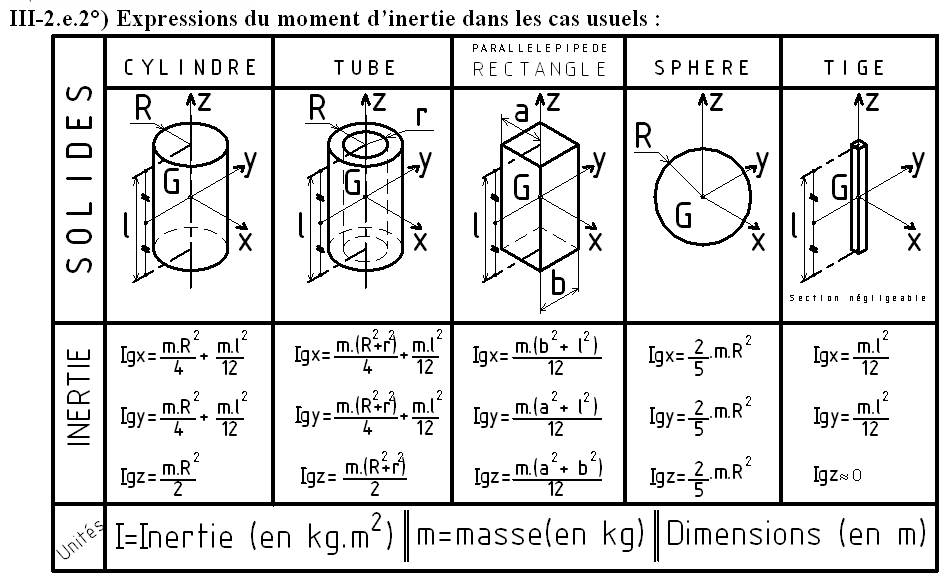
\includegraphics[scale=0.65]{MomentDinerties.png}
\end{center}


théorème de Huygens-Steiner

\medbreak

Rayon de giration
\begin{eqnarray}
I_G=m \cdot k_g^2 \Rightarrow k_G=\sqrt{\frac{I_G}{m}}\\
k^2=k_G^2+d^2
\end{eqnarray}



\subsection{Quantité mouvement, moment cinétique}
théorème quantité de mouvement : TAero, début Part 2\\
\begin{equation}
\iint_\Sigma [(\vec{p} \vec{n})+\rho \vec{V}(\vec{V} \vec{n})]d\sigma
\end{equation}
cette intégrale donne la force de poussée. \\
moment cinétique, théorème implusion\\
\url{https://fr.wikipedia.org/wiki/Quantit%C3%A9_de_mouvement}

	
	\newpage
	\section{Mécanique des structures}
	
	Loi de Hooke linéaire
	\begin{equation}
	F=k\cdot \Delta x
	\end{equation}
	
	\subsection{Traction/compression}
	\begin{equation}
	\sigma=\frac{F}{S}
	\end{equation}
	
	\begin{equation}
	\epsilon=\frac{\delta L}{l}
	\end{equation}
	
	\begin{equation}
	\epsilon=\frac{\sigma}{E}
	\end{equation}
	
	\subsection{Effort tranchant}
	\subsection{Flexion}
	
	\subsection{Torsion}
	
	Méthode flexion 3 points\\
	Poutre encastrée
	
	\subsection{Mécanique fluide}
	nombre de Reynolds
	\begin{equation}
	Re=V\cdot \frac{d \cdot \rho}{\eta}
	\end{equation}
	$V$ : vitesse $[m/s]$\\
	$d$ : dimension de l'objet $[m]$\\
	$\rho$ : masse volumique $[kg/m^3]$\\
	$\eta$ : viscosité en $[Pa \cdot s]$
	force frottement turbulant
	\begin{equation}
	\vec{F}_{fr}^{turbulant}=- \frac{1}{2} C_x \cdot \rho \cdot S \cdot \vec{v}^T \cdot \vec{v}
	\end{equation}
	$C_x$ : coefficient de traînée caractérisant la géométrie du solide, selon l'axe x\\
	
	force de frottement laminaire
	\begin{equation}
	\vec{F}_{fr}^{laminaire}=-k \cdot \eta \cdot \vec{v} 
	\end{equation}
	$k$ : coefficient caractéristique de la géométrie du solide\\
	$\eta$ : coefficient de viscosité du fluide (dépend de la température) $décapoise = N m^{-2}s = kg m^{-1}s^{-1}$
	
	finesse
	\begin{equation}
	f= \frac{C_z}{C_x}
	\end{equation}
	
	
	\subsection{Durée vie roulements}
	Efforts radiaux : $F_R$\\
	Efforts axiaux : $F_A$ \\
	\begin{equation}
	P=\sqrt{F_R^2+F_A^2}
	\end{equation}
	
	Vitesse de fonctionnement des roulements : $N$ en $tr/min$\\
	Durée de fonctionnement : $D$ en $h$\\
	Charge base d'un roulement : $C$ 
	
	\begin{eqnarray}
	L_{10}=N \cdot 60 \cdot D\\
	L_{10}=(\frac{C}{P})^3
	\end{eqnarray}
	
	
	
	\newpage
	\section{Mécanique vibratoire}
	modèle simple, pendule simple, amortissement, equation différentielle, solutions réelles, solutions complexes, ....
	exercice suspension vhc : système roue amortisseur/ressort -> fonction de transfert
	
	\subsection{Système à un degré de liberté}
	
	Ocillateur simple : une masse avec un ressort et un amortissement
	
	Equation du mouvement :
	\begin{equation}
	m \ddot{x} + c \dot{x}+k x =0
	\end{equation}
	qu'on peut écrire différemment. 
	\begin{equation}
	\ddot{x} + 2\zeta \omega_0 \dot{x}+\omega_0^2  x =0
	\end{equation}
	
	\begin{eqnarray}
	\omega_0=\sqrt{\frac{k}{m}}\\
	\zeta=\frac{c}{c_r}\\
	c_r=2 m \omega_0=2\sqrt{km}
	\end{eqnarray}
	$c_r$ : constante d'amortissement critique. 
	
	Solution : $x(t)=C \exp^{\lambda t}$
	
	\newpage
	\section{Statistique}
	\subsection{Combinatoire}
	Combinaison : 
	\begin{equation}
	C(x,y)=\begin{bmatrix}
	x\\
	y
	\end{bmatrix}=\frac{x!}{(x-y)!\cdot y!}
	\end{equation}
	
	
	Permutation
	\begin{equation}
	P(x)=x!
	\end{equation}
	Répartition d'un groupe de x dans des groupes de y et z éléments.
	
	\begin{eqnarray}
	x=y+z\\
	P^x_{y,z}=\frac{x!}{y! \cdot z!}
	\end{eqnarray}
	\subsection{***********}
	
	moyenne
	\begin{equation}
	\mu=\sum x_i \cdot P_i
	\end{equation}
	
	\begin{equation}
	\mu = \frac{1}{n}\sum x_i
	\end{equation}
	
	variance
	\begin{equation}
	v=\sum (x_i-\mu)^2\cdot P_i
	\end{equation}
	\begin{equation}
	v=\frac{1}{n} \sum (x_i-\mu)^2
	\end{equation}
	écart-type
	\begin{equation}
	\sigma=\sqrt{v}=\sqrt{\sum (x_i-\mu)^2\cdot P_i}
	\end{equation}
	
	Espérance (cas discret)
	\begin{equation}
	E(X)=\mu=\sum_{i=1}^{n}x_i\cdot P_i
	\end{equation}
	Jeu équitable si $E(X)=0$. avec bénifice $E(X)>0$
	
	\newpage
	\section{Régulation}
	
	Laplace, Fonction de transfert, Boucle de régulation : ouverte, fermée
	
	\newpage
	\section{Thermodynamics}
	\subsection{Définitions}
	Loi des gaz parfaits
	\begin{eqnarray}
	PV=nRT\\
	Pv=rT
	\end{eqnarray}
	$P$ : Pression du gaz $[Pa]$\\
	$V$ : Volume du gaz $[m^2]$\\
	$v$ : Volume spécifique $[\frac{m^2}{kg}]$\\
	$n$ : nombre de mole $[mol]$\\
	$R$ : Constante des gaz 8.314 $[\frac{J}{K \cdot K}]$\\
	$r$ : Constante massique d'un gaz \\
	$T$ : Température $[K]$\\
	
	
	Equation de Van der Waals :
	\begin{equation}
	p \cdot (V-)=n R T
	\end{equation}
	
	Energie interne d'un gaz :
	\begin{equation}
	U=\frac{\nu}{2} nRT=\frac{\nu}{2} N k_B T
	\end{equation}
	$\nu$ : 
	$k_B$ : constante de Bolzmann\\
	$N$ :  nombre de molécules\\
	
	Travail et travail massique:
	\begin{eqnarray}
	\delta W=\int_{min}^{max} p dV\\
	\delta w=\frac{\delta W}{m} =\int_{min}^{max} p dv\\
	\end{eqnarray}
	
	Chaleur et chaleur massique: 
	\begin{eqnarray}
	\delta Q=m*C_p*\Delta T\\
	\delta q= \frac{\delta Q}{m} C_p* \Delta T
	\end{eqnarray}
	
	Masse molaire :
	\begin{equation}
	M=\frac{m}{n}
	\end{equation}
	
	Rapport isentropique : rapport des chaleurs spécifiques
	Lois de Meyer :
	\begin{equation}
	\gamma=\frac{C_p}{C_v}=\frac{c_p}{c_v}
	\end{equation}
	\begin{equation}
	R=C_p-C_v
	\end{equation}
	On peut en déduire :
	
	\begin{equation}
	r=c_p-c_v
	\end{equation}
	
	\begin{eqnarray}
	c_p=\frac{C_p}{M}\\
	c_v=\frac{C_v}{M}
	\end{eqnarray}
	
	Pression partielle et pression totale (lois de Dalton):
	\begin{eqnarray}
	p_i \cdot V=n_i \cdot R \cdot T\\
	p=\sum p_i
	\end{eqnarray}
	
	\subsection{Principes de la thermodynamique}
	Premier principe :\\
	en présenced'un apport de chaleur $Q$ et de travail $W$, l'énergie interne d'un système change d'une valeur initiale $U_i$ à une valeur finale $U_f$. 
	\begin{equation}
	dU=\delta Q + \delta W
	\end{equation}
	
	\begin{eqnarray}
	\delta W = - p dV\\
	\delta Q = m \cdot c \cdot \Delta T 
	\end{eqnarray}
	Deuxième principe ou principe de Carnot :
	
	
	1er, 2ème, 3ème principe
	\subsection{Enthalpie (à contrôler)}
	Fonction d'état
	\begin{eqnarray}
	H = U + p \cdot V \\
	h = u + p \cdot v
	\end{eqnarray}
	isobare : $p \cdot \Delta V = 0$
	\begin{eqnarray}
	\Delta H = Q
	\end{eqnarray}
	\subsubsection{Enthalpie des gaz parfaits} 
	\begin{eqnarray}
	\Delta H = m \cdot c_p \cdot \Delta T\\
	\Delta h = c_p \cdot \Delta T\\
	\Delta U = m \cdot c_v \cdot \Delta T\\
	\Delta h = c_p \cdot \Delta T\\
	\end{eqnarray}
	\begin{eqnarray}
	H = U + p \cdot V = U + n \cdot R \cdot T\\
	h = u + p \cdot v = u + n \cdot r \cdot T
	\end{eqnarray}
	
	\begin{eqnarray}
	\Delta H = \Delta U + p \cdot \Delta V\\
	m \cdot c_p \cdot \Delta T = m \cdot c_v \cdot \Delta T + n \cdot R \cdot \Delta T\\
	\end{eqnarray}
	Simplification
	\begin{equation}
	c_p =  c_v  + r\\
	\gamma = \frac{c_p}{c_v}\\
	c_v = \frac{n \cdot R}{\gamma -1}\\
	c_p = \frac{n \cdot R \cdot \gamma}{\gamma -1}
	\end{equation}
	\subsubsection{Enthalpie des solides et des liquides}
	La pression est sans influence sur les solides et les liquides, en première approximation
	\begin{eqnarray}
	H ~= U\\
	c_p =~ c_v =~ c
	\end{eqnarray}
	\subsection{Entropie}
	Fonction d'état.\\
	Interprétation du second principe\\
	Système fermé : l'inégalité suivante est vérifiée : $dS >= \frac{\delta Q}{T_e}$
	\begin{equation}
	dS = \delta S_{échange}+ \delta S_{créée}= \frac{\delta Q}{T_e}+ \delta S_{créée}
	\end{equation}
	avec $\delta S_{créée} >= 0$
	\begin{equation}
	\Delta S =S_{échange}+S_{créée}= \int \frac{\delta Q}{T_e}+S_{créée}
	\end{equation}
	avec $ S_{créée} >= 0$
	
	Transformations réversible d'un système fermé: 
	\begin{eqnarray}
	dU = \delta Q_{rév} + \delta W_{rév} = \delta Q_{rév} - p \cdot d V\\
	dS = \delta S_{échange} + \delta S_{créée} = \frac{\delta Q_{rév}}{T} + 0\\
	\delta Q_{rév} = T \cdot dS
	\end{eqnarray}
	Premier principe
	\begin{equation}
	dU = T \cdot dS - p \cdot dV
	\end{equation}
	\subsubsection{Entropie  des gaz parfaits}
	\begin{eqnarray}
	dS = \frac{dU}{T} - \frac{p \cdot dV}{T}\\
	dS = c_v \frac{dT}{T} + n \cdot R \frac{dV}{V}
	\end{eqnarray}
	
	\begin{eqnarray}
	\Delta S^{gaz parfait}=S_2 - S_1 = c_v \cdot ln(\frac{T_2}{T_1})+ n \cdot R \cdot ln(\frac{V_2}{V_1})\\
	\Delta S^{gaz parfait}=S_2 - S_1 = c_p \cdot ln(\frac{T_2}{T_1})- n \cdot R \cdot ln(\frac{p_2}{p_1})
	\end{eqnarray}
	\subsubsection{Entropie des solides et des liquides}
	pression sans influence en première approximation
	\begin{eqnarray}
	\Delta S^{liquide}=S_2 - S_1 = c^{liquide} \cdot ln(\frac{T_2}{T_1})\\
	\Delta S^{solide}=S_2 - S_1 = c^{solide} \cdot ln(\frac{T_2}{T_1})
	\end{eqnarray}
	\subsection{Processus thermodynamiques}
	Equation des gaz parfaits 
	\begin{eqnarray}
	p \cdot V = n \cdot R \cdot T\\
	\end{eqnarray}
	Wan der Vaals
	\subsubsection{isobare}
	Pression constante 
	\begin{eqnarray}
	p_i = p_f = p -> \\
	\frac{V_i}{n_i \dot R \cdot T_i} = 	\frac{V_f}{n_f \dot R \cdot T_f}
	\end{eqnarray}
	Système fermé : $n_i=n_f$
	\begin{eqnarray}
	\frac{V_i}{T_i} = 	\frac{V_f}{T_f}
	\end{eqnarray}
	travail
	\begin{eqnarray}
	W = - \int p \cdot dV = p (V_f - V_i)
	\end{eqnarray}
	Pour une transformation isobare réversible d'un gaz parfait : 
	\begin{eqnarray}
	dS = \frac{c_p}{T} dT\\
	S = \int dS = \int \frac{c_p}{T} dT\\
	S = c_p \cdot ln(T) + B\\
	T = e^{\frac{S-B}{c_p}} = k \cdot e^{\frac{S}{c_p}}
	\end{eqnarray}
	$B$ est une constante définie par les conditions initiales du systèmes. De plus, une translation à température constante est définie par : 
	\begin{equation}
	MM'=S'-S=r \cdot ln(\frac{v}{v'})
	\end{equation}
	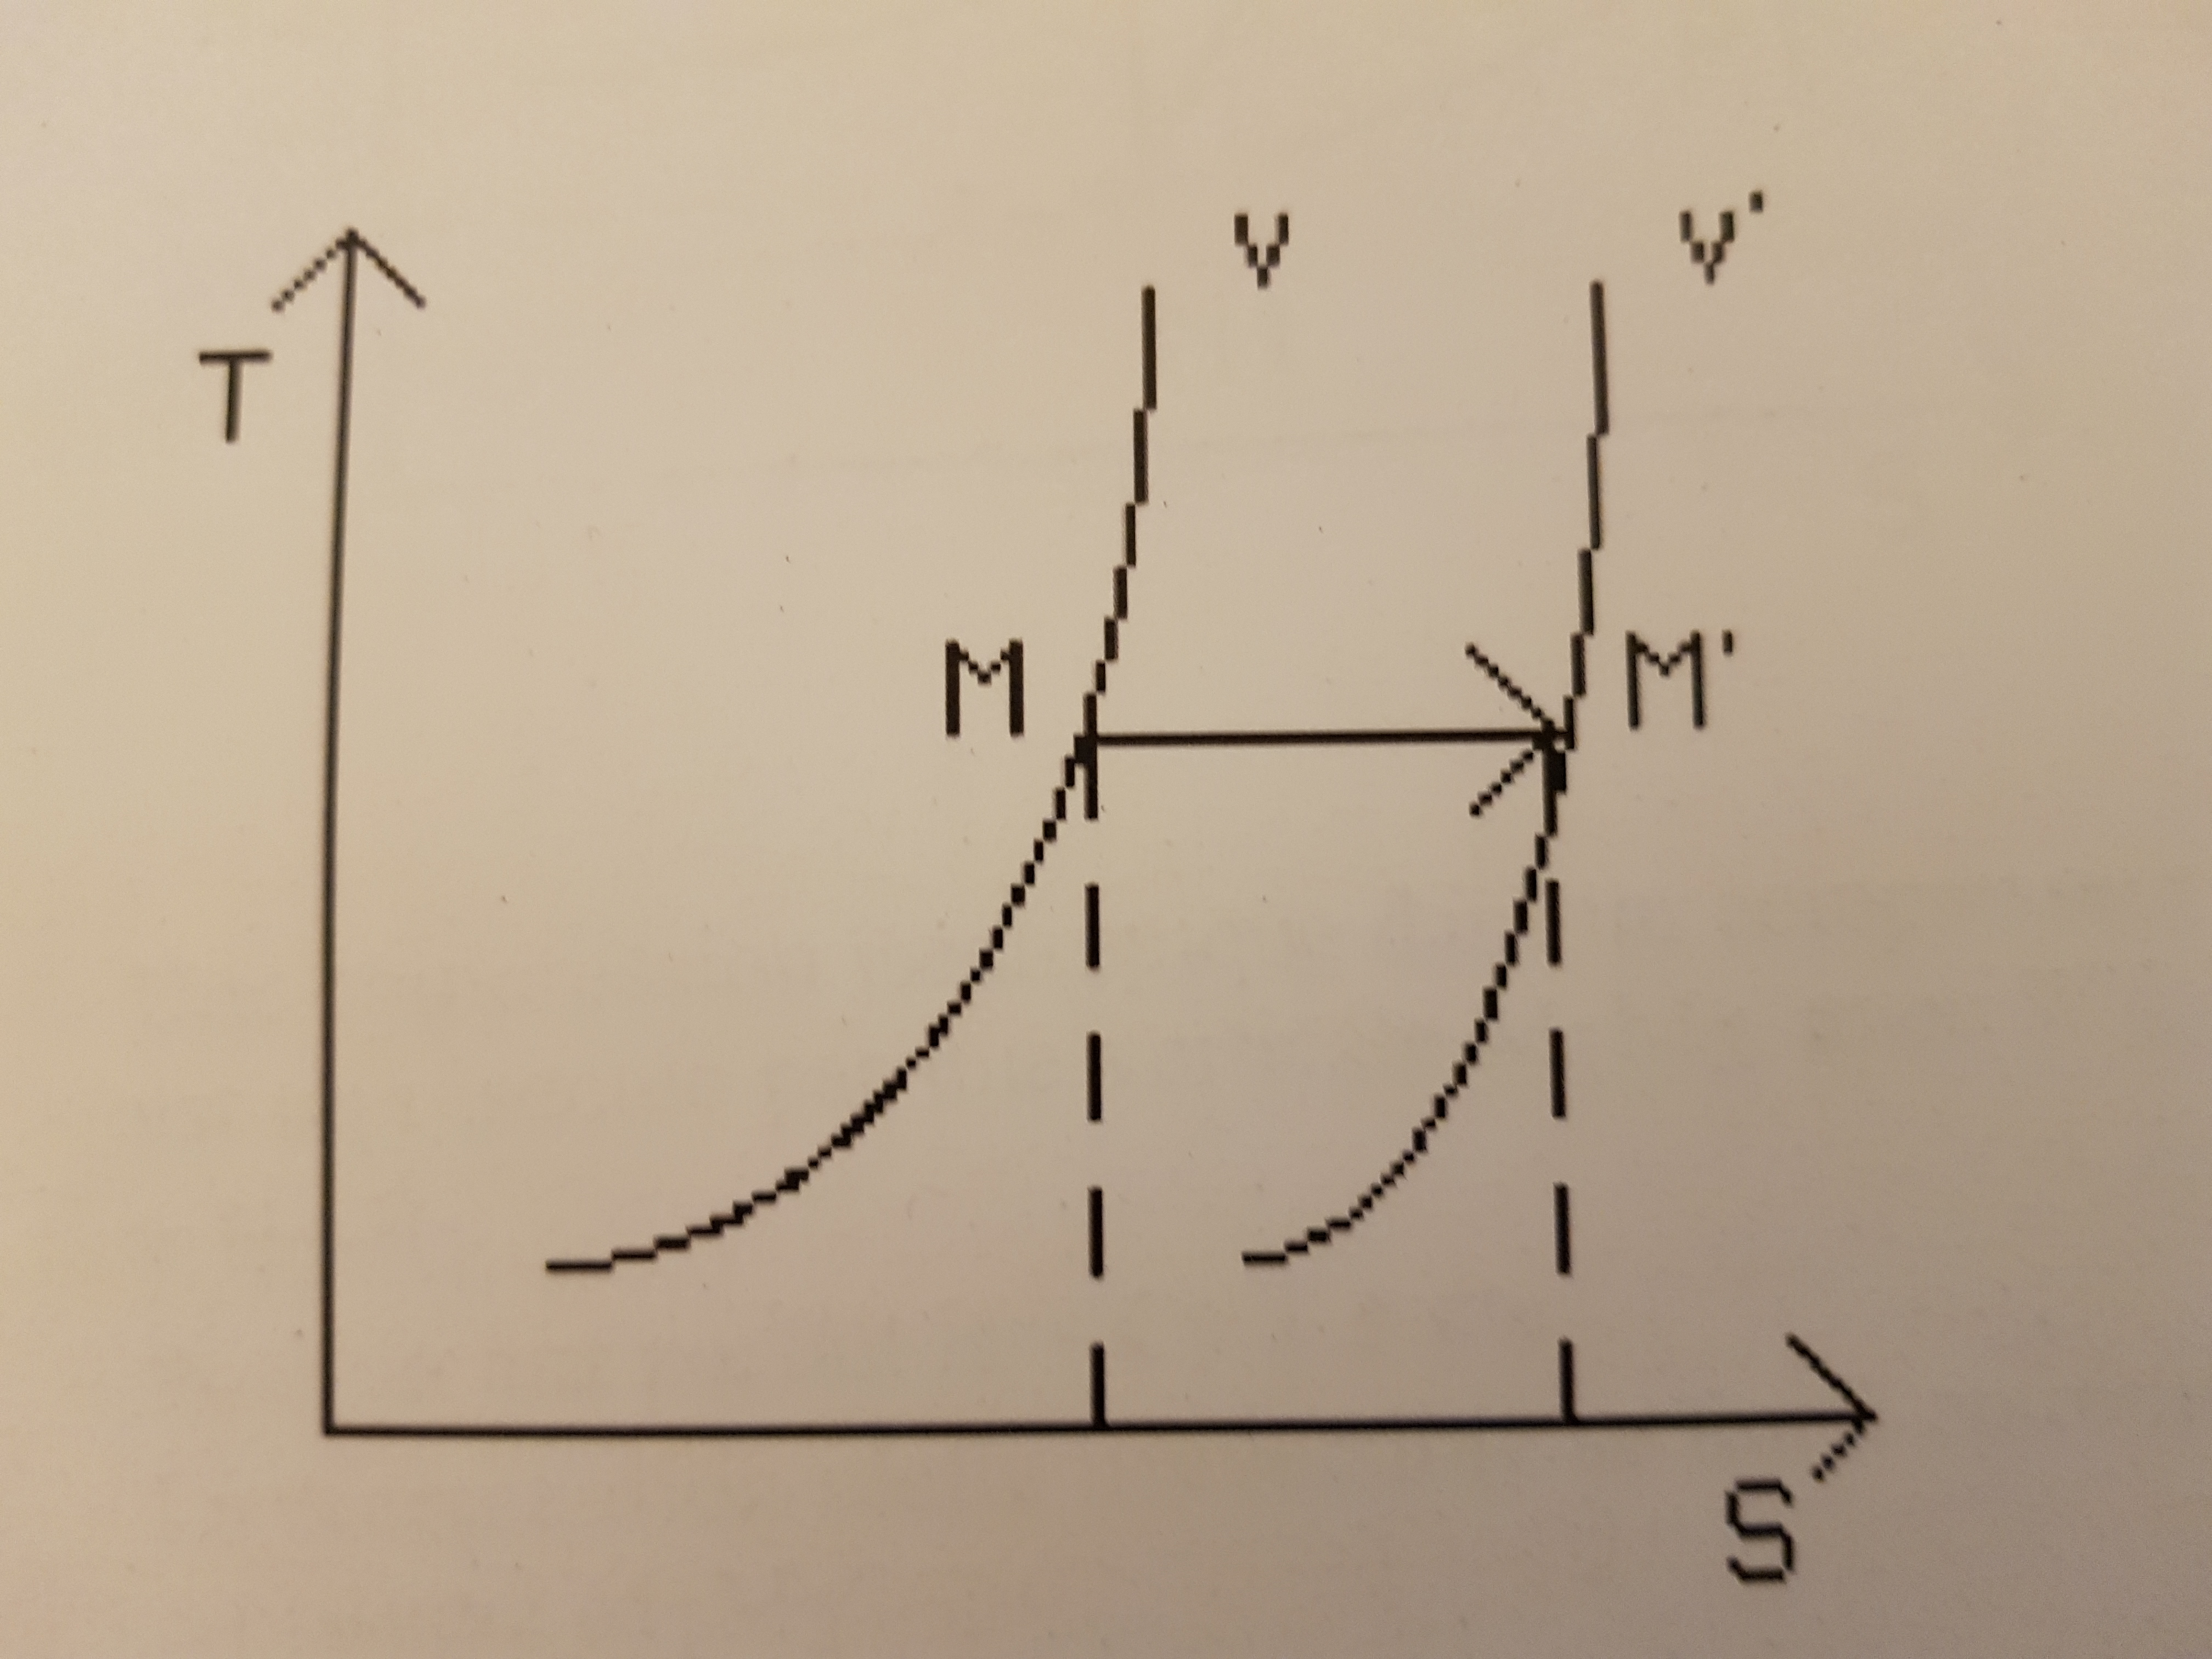
\includegraphics[scale=0.1]{isochoric_t_s.jpg}
	
	Dans les diagrammes P-V et T-S, une transformation isochore d'un gaz parfait est représentée par une exponentielle. \\
	
	% 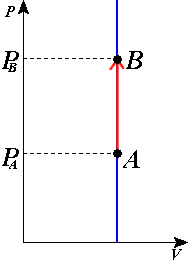
\includegraphics[scale=0.6]{Isochoric_process_P_V.png}\\
	
	% 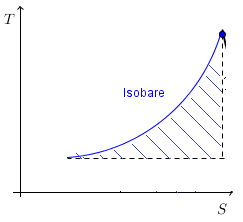
\includegraphics[scale=1]{Isochoric_process_T_S.png}
	\subsubsection{isotherme}
	Température constante.
	
	\begin{eqnarray}
	T_i = T_f = T -> \\
	\frac{p_i \cdot V_i}{n_i \dot R} = 	\frac{p_f \cdot V_f}{n_f \dot R}
	\end{eqnarray}
	
	Système fermé : $n_i=n_f$
	\begin{eqnarray}
	p_i \cdot V_i = p_f \cdot V_f
	\end{eqnarray}
	Travail 
	\begin{eqnarray}
	W = - \int p \cdot dV\\
	W = - \int \frac{n \cdot R \cdot T}{V} \cdot dV\\
	W = - n \cdot R \cdot T ln(\frac{V_f}{V_i})
	\end{eqnarray}
	\subsubsection{isochore}
	Volume constant 
	\begin{eqnarray}
	V_i = V_f = p -> \\
	\frac{p_i}{n_i \dot R \cdot T_i} = 	\frac{p_f}{n_f \dot R \cdot T_f}
	\end{eqnarray}
	
	Système fermé : $n_i=n_f$
	\begin{eqnarray}
	\frac{p_i}{T_i} = 	\frac{p_f}{T_f}
	\end{eqnarray}
	
	Pour une transformation isochore réversible d'un gaz parfait : 
	\begin{eqnarray}
	dS = \frac{c_v}{T} dT\\
	S = \int dS = \int \frac{c_v}{T} dT\\
	S = c_v \cdot ln(T) + B\\
	T = e^{\frac{S-B}{c_v}} = k \cdot e^{\frac{S}{c_v}}
	\end{eqnarray}
	$B$ est une constante définie par les conditions initiales du systèmes.
	Dans le diagramme P-V, une transformation isochore d'un gaz parfait est représentée par une droite verticale. \\
	
	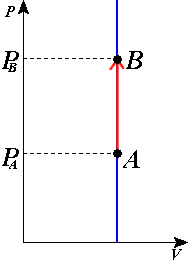
\includegraphics[scale=0.8]{Isochoric_process_P_V.png}\\
	
	Dans le diagramme T-S, une transformation isochore d'un gaz parfait est représentée par une exponentille. 

	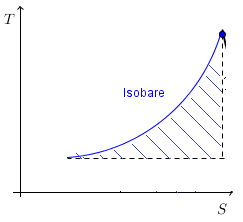
\includegraphics[scale=1.4]{Isochoric_process_T_S.png}
	
	\subsubsection{adibatique}
	Pas d'échange de chaleur avec l'extérieur : système isolé, parfaitement calorifugé
	\begin{eqnarray}
	p \cdot V^\gamma = constante_1\\
	T \cdot V^{\gamma-1}=constante_2\\
	T \cdot p^{\frac{1-\gamma}{\gamma}}=constante_3
	\end{eqnarray}
	\subsubsection{polytropique}
	processus adiabatique, mais réel, donc avec échange de chaleur
	\subsubsection{Tableau résumé}
	\begin{tabular}{|l|c|c|c|c|c|}
		\hline
		Processus & Formules & $\delta w$ & $\delta q$ & U & Particularités \\ \hline
		isochore & $\Delta v=0$, $\frac{r*T}{p}=const$ & 0 & & & \\ \hline
		isobare & $\Delta p=0$,$\frac{rT}{v}=const$ & $-p_0 \cdot (v_1-v_0)$ & & & \\ \hline
		isotherme & $\rho$ & 7860 $\frac{kg}{m^3}$ & & &\\ \hline
		adiabatique & $\alpha$ & & & & Un processus est adibatique quand il n'y pas d'échange de chaleur entre le système et l'extérieur. \\ \hline
		isentrope & $p*V^\gamma=const$, $T^\gamma*p^{1-\gamma}=const$, $
		T*V^{\gamma-1}=const$ & & $\delta Q=0$ & & adiabate sans pertes \\ \hline
		polytropique & $\sigma=...$ & & & & \\ \hline
	\end{tabular}
	\medbreak
	Facteur polythroqique : $\sigma$
	
	Polythropic Processus : general law for the expansion and compression of gases
	
	\begin{equation}
	p \cdot V^{\sigma}=const
	\end{equation}
	
	Heat absorbed or rejected during a polythropic process :
	\begin{equation}
	\begin{split}
	Q=\frac{\gamma - \sigma}{\gamma - 1} \cdot Workdone = \frac{\gamma - \sigma}{\gamma - 1} \cdot \frac{p_1 v_1 - p_2 v_2}{\sigma-1}\\= 
	\frac{\gamma - \sigma}{\gamma - 1} \cdot \frac{m R (T_1 -T_2)}{\sigma-1}=\frac{\gamma - \sigma}{\gamma - 1} \cdot m c_{\gamma} (T_1 -T_2)
	\end{split}
	\end{equation}
	\begin{equation}
	n = \frac{log(p_2/p_1)}{log(v_1/v_2)}
	\end{equation}
	
	Notes :
	\begin{itemize}
		\item when $\sigma < \gamma$, the heat is absorbed by the gas
		\item when $\sigma > \gamma$, the heat is rejected by the gas
	\end{itemize}
	
	\subsection{Cycles}
	Carnot, Rankine, Lenoir, diesel, diesel pour Wankel, Otto,   .... avec les rendements 
	
	Dans un moteur, le transfert de chaleur se fait dans le sens spontané, du chaud vers le froid : $Q_c > 0$ et $Q_f <0$. on récupère le travail, donc $W <0$. 

	\begin{equation}
	\eta = \frac{grandeur utile}{grandeur couteuse}= \frac{\abs W}{Q_c}
	\end{equation}
	Sachant que : 
	\begin{eqnarray}
	\abs W = - W = Q_c + Q_f\\
	\frac{Q_c}{T_c} + \frac{Q_f}{T_f} <= 0\\
	- \frac{T_f}{T_c} <= \frac{Q_f}{Q_c}
	\end{eqnarray}
	
	\begin{eqnarray}
	\eta = \frac{\abs W}{Q_c} = \frac{Q_c + Q_f}{Q_c} = 1+ \frac{Q_f}{Q_c} \\
	\eta <= 1 - \frac{T_f}{T_c}
	\end{eqnarray}
	Ceci est la borne supérieur pour le rendement. C'est le théorème de Carnot. 
	
	\subsubsection{Carnot}
	2 isothermes, 2 isentropes : (ajouter schéma dans diagramme Ts et pv)
	
	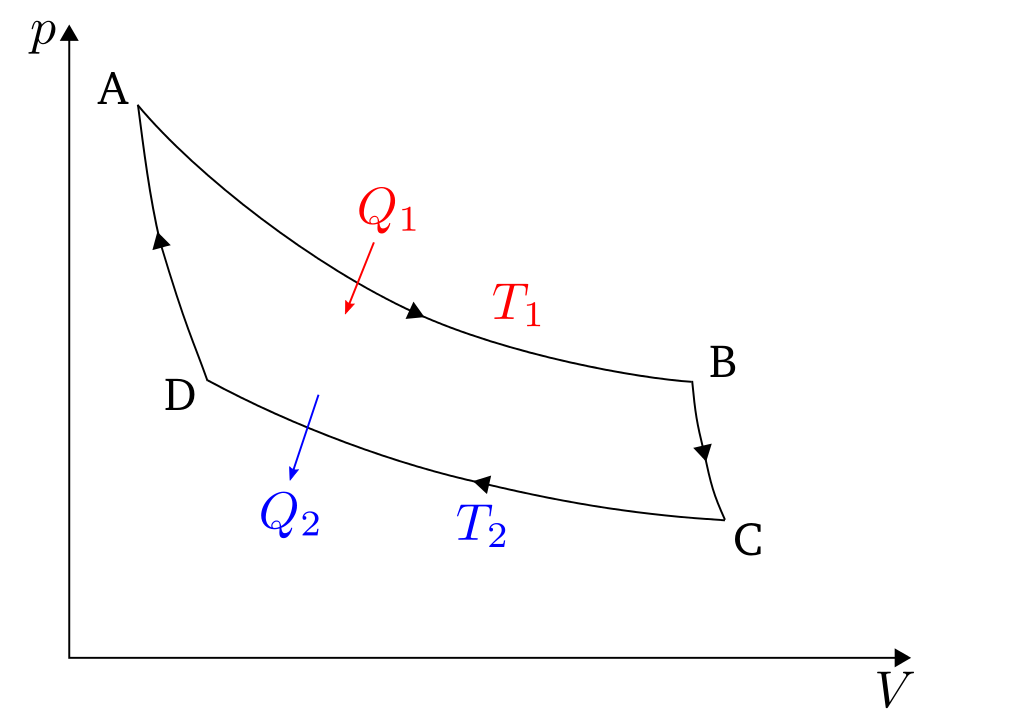
\includegraphics[scale=0.3]{Carnot_cycle_p_V_diagram.png}
	
	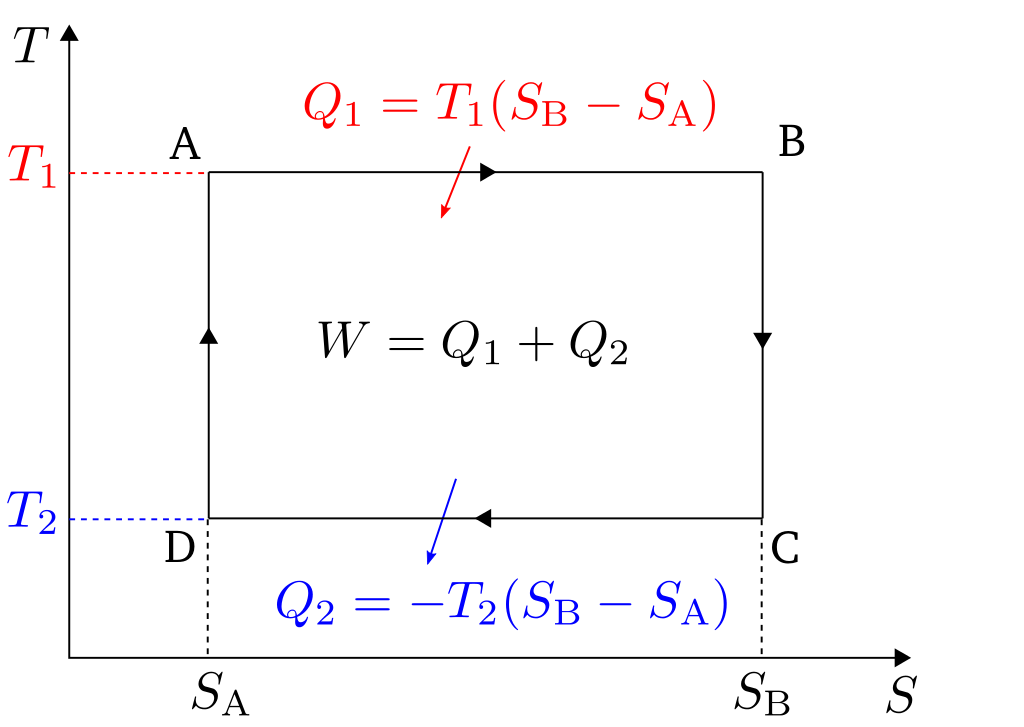
\includegraphics[scale=0.3]{Carnot_cycle_T_S_diagram.png}

	l'aire $A = T \cdot dS$ est égale à la quantité de chaleur échangée au cours de cette transformation. De manière générale, cette aire est égale au travail et à la chaleur échangés.
	\subsubsection{Otto}
	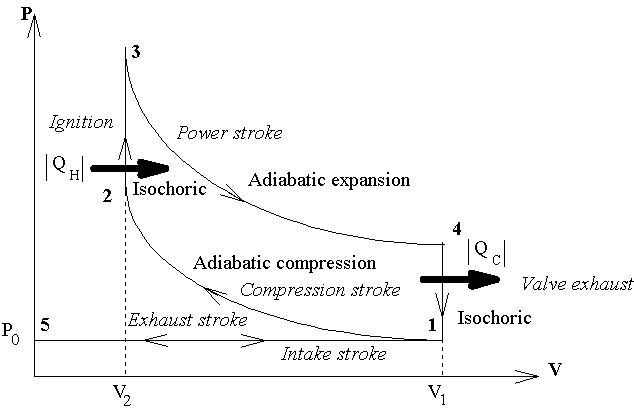
\includegraphics[scale=1]{otto_cycle.png}
	A thermodynamic cycle is used in internal combustion engine using gasoline/petrol as fuel. It's name comes from the german engineer Otto, who invented this type of engine in 1861. 
	\medbreak
	This cycle is composed of 4 strokes : 
	\begin{enumerate}
		\item Intake\\
	The intake valve opens and the air-fuel mixture is drawn into the cylinder at nearly atmospheric pressure as the piston moves downward. When the piston start to move back up, the intake valve is closed.
	
	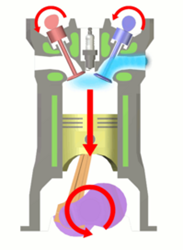
\includegraphics[scale=1]{otto_Intake_stroke.png}
		\item Compression\\
	In this stroke, the intake and the exhaust valves are closed. As the piston moves upward, the pressure in the cylinder rises and the air-fuel mixture is compressed.
	
	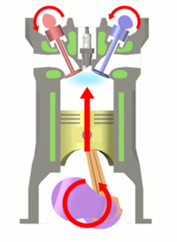
\includegraphics[scale=1]{otto_Compression_stroke.png}
		\item Explosion/Power\\
	The mixture is ignited by the spark plugs at a position where the piston position is nearly fixed. The temperature and the pressure rise rapidly due to the ignition. Then the ignited hot gas pushed the piston downward allowing to do the mechanical work.
	
	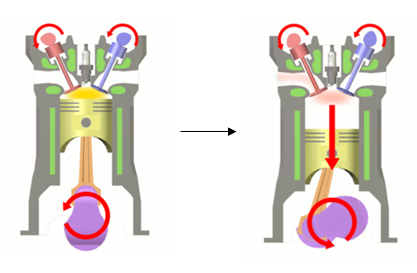
\includegraphics[scale=1]{otto_Power_Stroke.png}
		\item Exhaust\\
	The exhaust valve is opened and as the piston moves upward again, the ignited gas escapes through the exhaust valve.
	 
	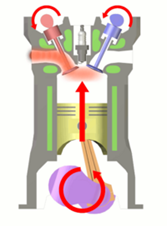
\includegraphics[scale=1]{otto_Exhaust_Stroke.png}
	\end{enumerate}
	
	
	\medbreak
	\url{http://www.zoombd24.com/otto-cycle-strokes-thermodynamic-processes-p-v-and-t-s-diagram-and-efficiency/}
	\subsubsection{Diesel}
	\subsubsection{Diesel for Wankel engine}
	\subsection{Rendements isentropiques}
	
	Rendement de Carnot
	
	Rendement isentropique d'un compresseur :
	
	\begin{equation}
	\eta_c=\frac{\Delta H_s}{\Delta H_r}=\frac{Cp*(T_s-T)}{Cp*(T_r-T)}
	\end{equation}
	
	Rendement isentropique d'une turbine :
	
	\begin{equation}
	\eta_t=\frac{\Delta H_r}{\Delta H_s}
	\end{equation}
	
	\subsection{Afterburner}
	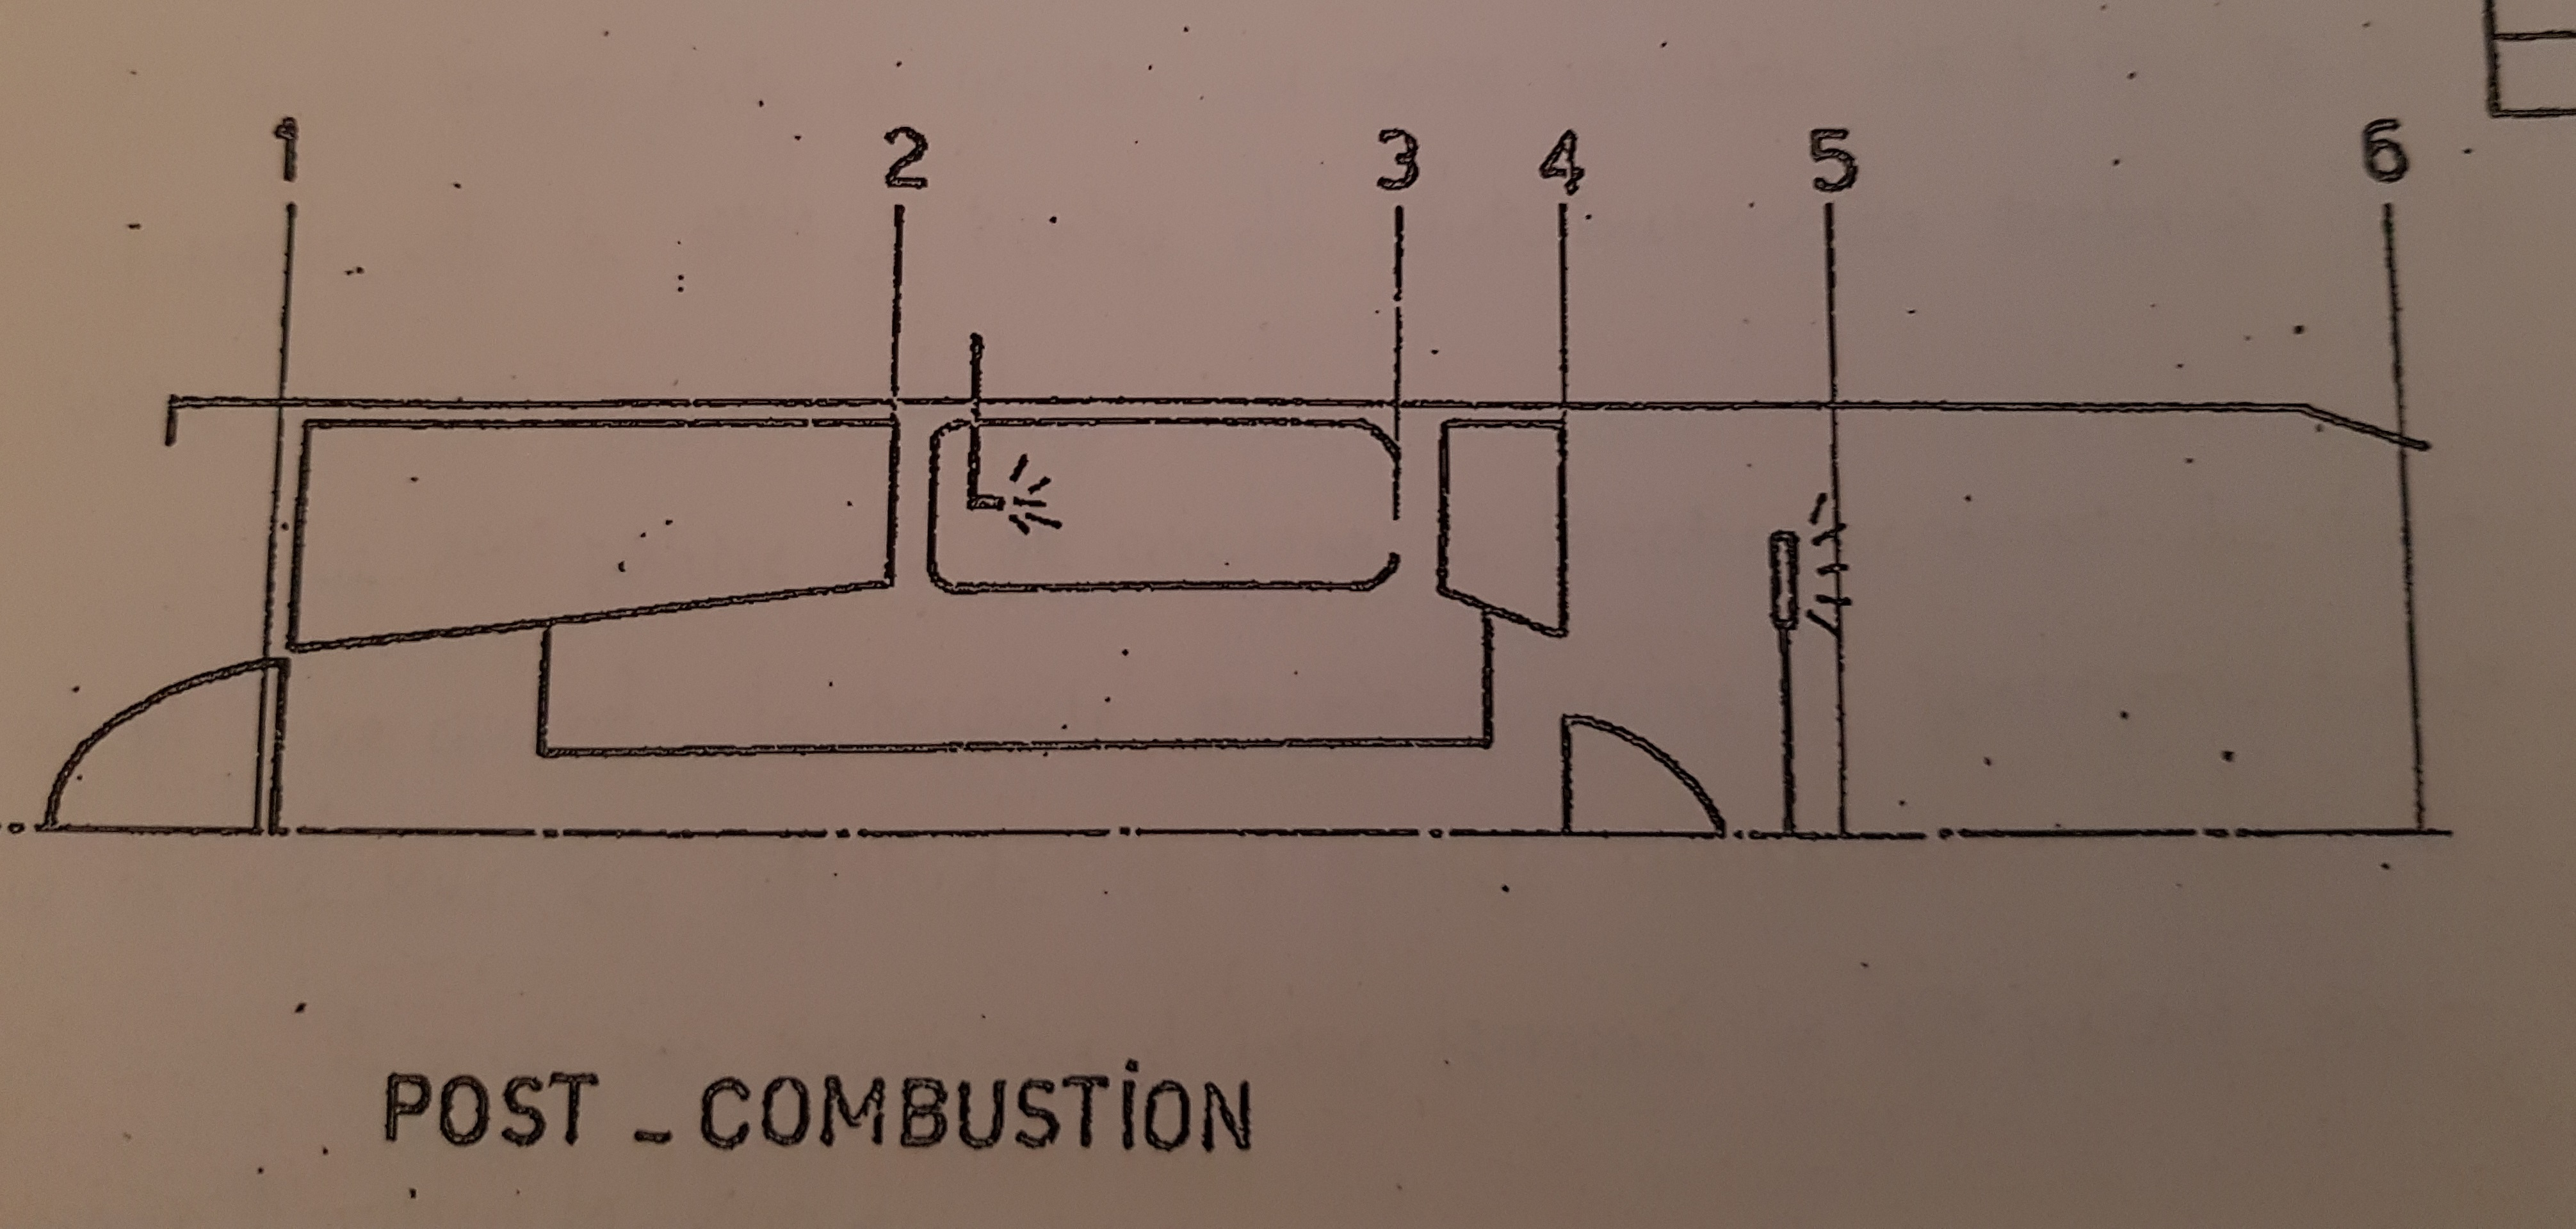
\includegraphics[scale=0.1]{Afterburner_schema.jpg}
	\\
	1 : entrée compresseur\\
	2 : entrée chambre de combustion\\
	3 : entrée turbine\\
	4 : sortie turbine \\
	5 : entrée post-combustion\\\\
	6 : sortie tuyère\\
	
	\begin{equation}
	\frac{F}{q \cdot \sqrt{T_{i1}}}=(1+m) \cdot \sqrt{2 \cdot C_p \cdot \frac{T_{i5}}{T_{i1}}\cdot[1-(\frac{P_0}{P_{i5}})^{\frac{\gamma-1}{\gamma}}]}-\frac{V_0}{\sqrt{T_{i1}}}
	\end{equation}
	
	\begin{equation}
	V_0^2 = 2 \cdot C_p \cdot T_{cp} \cdot [1-(\frac{P_0}{P_{i4}})^{\frac{\gamma-1}{\gamma}}]
	\end{equation}
	
	\begin{equation}
	\frac{F}{q \cdot \sqrt{T_{l1}}}=(1+m) \cdot \sqrt{2 \cdot C_p \cdot \frac{T_{i5}}{T_{i1}}\cdot[1-(\frac{P_0}{P_{i6}})^{\frac{\gamma-1}{\gamma}}]}-\frac{V_0}{\sqrt{T_{i1}}}
	\end{equation}
	
	F : force de poussée. (étudier les unités pour reconnaître les paramètres)
	\subsection{Rayonnement corps noir}
	Puissance rayonnée :
	\begin{equation}
	P= \sigma * T^4
	\end{equation}
	$P$ : puissance rayonnée $[W]$\\
	$T$ : température $[T]$\\
	$\sigma$ : 
	
	\subsection{Changement de phase}
	Energie de changement de phase
	\begin{eqnarray}
	\delta Q=L \cdot \delta m\\
	Q=L \cdot m
	\end{eqnarray}
	$L$ : chaleur latente de fusion/évaporation $[\frac{J}{kg}]$\\
	Remarque : lors du changement de phase, la température reste constante. Toute l'énergie absorbe est utilisée pour le changement de phase.
	
	Hors des phases, l'énergie augmente la température. L'énergie interne change selon la relation suivante : 
	\begin{equation}
	dU=\delta Q=m*C_x*\Delta T
	\end{equation}
	
	
	
	
	\newpage
	\section{Conversion d'unité}
	
	1mmHg=133.3 Pa\\
	1 atm=1013.25 hPa = 760 torr\\
	
	Équations conversion Kelvin (K), Celcius (C) et Fahrenheit (F).
	
	\begin{equation}
	K=C+273.15
	\end{equation}
	
	
	\newpage
	\section{Bibliographie}
	Liste des cours, avec le nom des profs\\
	liste des livres\\
	+ sources diverses

\end{document}